% CVPR 2022 Paper Template
% based on the CVPR template provided by Ming-Ming Cheng (https://github.com/MCG-NKU/CVPR_Template)
% modified and extended by Stefan Roth (stefan.roth@NOSPAMtu-darmstadt.de)

\documentclass[10pt,twocolumn,letterpaper]{article}

%%%%%%%%% PAPER TYPE  - PLEASE UPDATE FOR FINAL VERSION
%\usepackage[review]{cvpr}      % To produce the REVIEW version
\usepackage{cvpr}              % To produce the CAMERA-READY version
%\usepackage[pagenumbers]{cvpr} % To force page numbers, e.g. for an arXiv version

% Include other packages here, before hyperref.
\usepackage{graphicx}
\usepackage{amsmath}
\usepackage{amssymb}
\usepackage{booktabs}
\usepackage{subcaption}
\usepackage{caption}
% It is strongly recommended to use hyperref, especially for the review version.
% hyperref with option pagebackref eases the reviewers' job.
% Please disable hyperref *only* if you encounter grave issues, e.g. with the
% file validation for the camera-ready version.
%
% If you comment hyperref and then uncomment it, you should delete
% ReviewTempalte.aux before re-running LaTeX.
% (Or just hit 'q' on the first LaTeX run, let it finish, and you
%  should be clear).
\usepackage[pagebackref,breaklinks,colorlinks]{hyperref}
\usepackage{multirow}


% Support for easy cross-referencing
\usepackage[capitalize]{cleveref}
\crefname{section}{Sec.}{Secs.}
\Crefname{section}{Section}{Sections}
\Crefname{table}{Table}{Tables}
\crefname{table}{Tab.}{Tabs.}


%%%%%%%%% PAPER ID  - PLEASE UPDATE
\def\cvprPaperID{*****} % *** Enter the CVPR Paper ID here
\def\confName{CVPR}
\def\confYear{2022}

\begin{document}

%%%%%%%%% TITLE - PLEASE UPDATE
\title{Open-Set Domain Adaptation through Self-Supervision}

\author{Protopapa Andrea, Quarta Matteo, Ruggeri Giuseppe, Versace Alessandro\\
Politecnico di Torino\\
Italy\\
{\tt\small \{s286302,s292477,s292459,292435\}@studenti.polito.it}
% For a paper whose authors are all at the same institution,
% omit the following lines up until the closing ``}''.
% Additional authors and addresses can be added with ``\and'',
% just like the second author.
% To save space, use either the email address or home page, not both
}
\maketitle

%%%%%%%%% ABSTRACT
\begin{abstract}
  In machine learning applications, domain adaptation (DA) techniques try to mitigate the problem of having different domains in the training and test data.
  Another common problem is represented by the presence of more semantic classes in the test data, which are unknown
  and completely new to the developed models. The latter problem comes under the name of novelty or anomaly detection.
  In real world scenarios, it is becoming extremely common suffering of both problems.
  \textit{Open-Set Domain Adaptation (OSDA)} methods try to tackle these problems by jointly adapting a model trained on a labeled source domain to an unlabeled target domain
  while performing novelty detection. We propose a new method leveraging a self-supervised technique, rotation recognition, constisting in first performing
  novelty detection on the target data and then aligning the two domains avoiding potential negative adaptation.
  Furthermore, we assess the performance using a new metric which represents in a balanced way the ability to jointly solve the two problems.
  Experiments conducted on the Office-Home benchmark show interesting results and method effectiveness.
   

  % Performance loss over domain change is a common problem in machine learning applications.
  % Solving the issue usually relies on adapting the model to the new domain by having at disposal large and labeled datasets, either rare or costly to acquire.
  % In this paper we propose a new approach, adapting models to the new domains while not needing relying on labeled data thanks to a self-supervision.
  % Experiments conducted on the Office-Home dataset show interesting results and method effectiveness.
\end{abstract}

\section{Introduction}
\label{sec:intro}
Nowadays, the widespread usage of deep neural networks to accomplish computer vision tasks has brought huge benefits.
In real world applications, as the tasks to cope with are becoming more and more challenging, machine learning methods commonly suffer of a gap between the performance
obtained during the development, and the actual performance observed in real usages. 

One of the problems which is causing this loss of performance is the domain gap between the training data and the actual observed data. Intuitively, if we train a model on a specific domain,
such as employing real world pictures depicting real objects, for example to perform classification, we expect that the model will perform well on a fairly large variety of test cases.
However, the actual data present a huge variety on the domains while still representing the same semantic classes that we want to predict.
For example, we may want to be capable of predicting that both an image of a real elephant and a drawing of an elephant are containing the semantic class \textit{elephant}.
Domain adaptation techniques have been developing in recent years to reduce the domain gap between a labeled source domain and one or more unlabeled target domains.
Generally, this is done by enforcing the learning of domain-invariant patterns of both domains.
As underlined in \cite{domainAdaptFarahani}, this is usually achieved by learning a transformation function which projects both the source and target domain data in a
new space where we jointly maintain the underlying structure of the original data while reducing the domain gap by removing the domain-specific information.

Another big issue encountered in real world usages is the presence of additional anomaly semantic classes on the observed data.
The problem comes under the name of \textit{Open-Set Recognition (OSR)} \cite{OSRsurvey}, where we require not only to accurately classify the known seen classes, but also
effectively deal with unknown ones, which would otherwise drastically weaken the robustness of the methods.

The jointly presence and accounting of the two described problems has been emerged as a new sub-field of computer vision with the name of \textit{Open-Set Domain Adaptation (OSDA)}.
As a consequence, if we try to reduce the domain gap between the whole target domain and the source domain, we will observe a negative adaptation due to the unwanted alignment between
the data belonging to the anomaly semantic classes and the source classes we want to model and predict.
For this reason, it is important to first perform anomaly detection of the additional set of novelty classes, translating the problem into a \textit{Closed-Set Domain Adaptation (CSDA)} one,
and next do the alignment between the source and the target domain identified as known.

Common machine learning methods usually leverage huge manually annotated datasets to perform well on the given tasks.
However, acquiring annotated material is usually very costly and difficult, moreover, relying on such data may not be scalable in large applications on the long run.
Thus, recently, a commonly employed approach is self-supervised learning, which consists in creating new automatically labeled data starting from the original unlabeled data.
The fundamental idea is creating some auxiliary task from input data so that,
by solving such task, the model can learn the underlying structure of the data,
for instance high-level knowledge, correlations, and metadata embedded.
This type of learning has been recently used for Domain Adaptation, 
learning robust cross-domain features and supporting generalization \cite{CarlucciJigsaw,SelfSupervisedXu},
and also for some Open Set problems specialized in anomaly detection and discriminating anomalous data \cite{bergman2020classificationbased,dectionGeometric}. 

The approach presented in this paper combines the power of the self-supervised learning with the standard supervised learning approach for semantic class recognition.
A two-stage method is hence proposed, 
aiming to identify and isolate unknown class samples in the first stage, 
before reducing in the second stage the domain gap between the source domain and the known target domain to avoid negative transfer.
This is done in both stages using a modified version of the rotation task as self-supervised method,
predicting the relative rotation between an image and its rotated version.
Finally, a classifier is used to predict if each target sample belongs either to one of the knwon classes or to an unknown class, 
being rejected in the latter case.
We evaluate the method on the Office-Home benchmark \cite{OfficeHomeDataset} exploiting a new OSDA metric. 

To wrap up, our \textbf{main contributions} are: 
\begin{enumerate}
  \item we define a new method to tackle OSDA problems which exploits the rotation recognition task to perform both the known/unknown target separation
and the domain adaptation;
  \item we introduce a new OSDA metric which properly balances the measure of both the performance on predicting the known classes and the performance on doing the unknown rejection;
  \item we conduct an extensive ablation over the hyperparameters for different variants of the self-supervised task underlying the benefits of some techniques over others.
\end{enumerate}


% Classical machine learning in the past years has made some oversimplified assumptions actually detached % Punteggiatura?
% from the usage of artificial intelligence systems in everyday real world and the problems they come with.

% The first assumption is that training and test sets come from the same distributions:
% a model trained on labeled data is expected to perform as well as on the test data.
% However, this assumption not always holds in real-world applications, 
% where naively applying the trained model on a new dataset may cause degradation in the performance.
% To solve this problem Domain Adaptation is widely used, 
% where the goal is to train a neural network on a source dataset for which labels are available and search for good performance on a target dataset, 
% which is related to but significantly different from the source dataset, 
% and whose label or annotation is not available. 
% Generally this is done by by minimizing the difference between domain distributions and enforcing the recognition of domain invariant patterns in both domains. 
% As underlined in \cite{domainAdaptFarahani}, 
% this is usually achieved by mapping source and target data by learning transformations for extracting such features and minimizing the gap between domains in the new representation space in an optimization procedure,
% while preserving the underlying structure of the original data. 

% Secondly, 
% in real-world classification tasks it is usually difficult to collect training samples to exhaust all classes when training a model.
% A more realistic scenario is open set recognition (OSR) \cite{OSRsurvey},
% where incomplete knowledge of the world exists at training time and unknown classes can be injected during testing, 
% requiring classifiers to not only accurately classify the seen classes but also effectively deal with unseen ones,
% which would otherwise drastically weaken the robustness of the methods.
% On the contrary this system should reject unknown classes at test time and separate the known and unknown samples.
% As underlined by \cite{OSRclassRec}, 
% existing open-set classifiers rely on deep networks trained in a supervised fashion on known classes in the training set;
% this causes specialization of learned representations to known classes and makes it hard to distinguish the unknowns from the knowns.

% To solve these significant issues our method is focused on a self-supervised task. 
% Self-supervised learning is an unsupervised learning technique where the supervised task is created out of the unlabeled input data. 
% This task could be as simple as predicting the lower half of an image being given the upper half of the same.
% Supervised learning requires both labeled and high quality data,
% usually very expensive, 
% whereas unlabeled data is often readily available in abundance.
% The fundamental idea behind self-supervised learning is creating some auxiliary task from input data so that,
% by solving such task,
% the model can learn the underlying structure of the data,
% for instance high-level knowledge, correlations, and metadata embedded in the data.
% This type of learning was recently used for Domain Adaptation, 
% learning robust cross-domain features and supporting generalization \cite{CarlucciJigsaw,SelfSupervisedXu},
% and also for some Open Set problems specialized in anomaly detection and discriminating anomalous data \cite{bergman2020classificationbased,dectionGeometric}.

% The approach presented in this paper brings these topics together in the so called Open-Set Domain Adaptation (OSDA) problem. 
% A two-stage method is hence proposed, 
% aiming to identify and isolate unknown class samples in the first stage, 
% before reducing in the second stage the domain gap between the source domain and the known target domain to avoid negative transfer.
% This is done in both stages using a modified version of the rotation task as self-supervised model,
% predicting the relative rotation between an image and its rotated version.
% Finally a classifier is used to predict if each target sample belongs either to one of the knwon classes or to an unknown class, 
% being rejected in the latter case.

% The method was evaluated on the Office-Home benchmark \cite{OfficeHomeDataset} with a specific OSDA metric.

% {\bf ADD HERE RESULTS AND A BRIEF OF CONCLUSIVE IDEAS (ALSO POSSIBLE FUTURE WORKS)!!}

%------------------------------------------------------------------------
\section{Related Work}
\label{sec:relatedwork}


\section{Method}
\label{sec:method}

\subsection{Problem Formulation}
\label{sec:problemformulation}
We define as $\mathcal{D}_s = \{({\bf x}_i^s, y_i^s)\}_{i=1}^{N_s} \sim p_s$ the source dataset whose distribution of samples and labels is $p_s$,
while $\mathcal{D}_t = \{{\bf x}_i^t\}_{i=1}^{N_t} \sim p_t$ is the unlabeled target dataset drawn from distribution $p_t$. 

The source dataset $\mathcal{D}_s$ is associated with a set of known classes $\mathcal{C}_s$,
whereas the target dataset $\mathcal{D}_t$ contains a set of classes $\mathcal{C}_t = \mathcal{C}_s \cup \mathcal{C}_{t \setminus s}$.
In other words,
$|\mathcal{C}_s| < |\mathcal{C}_t|$ and $\mathcal{C}_s \subset \mathcal{C}_t$. 

In OSDA we have that $p_s \neq p_t$.
Moreover, it holds that $p_s \neq p_t^{\mathcal{C}_s}$, where $p_t^{\mathcal{C}_s}$ denotes the distribution of the target domain if we restrict to
the shared classes $\mathcal{C}_s$. 

Summarizing, in OSDA tasks, we have both a domain gap ($p_s \neq p_t^{\mathcal{C}_s}$)
and a category gap ($\mathcal{C}_s \neq \mathcal{C}_t$). Moreover, the goal is to assign the target samples either to a category ${i \in \mathcal{C}_s}$,
or to reject them as {\it unknown}.
A metric to measure the complexity of an OSDA problem is the {\it openness} betweeen the source and the target domain \cite{bendale2015open}, 
defined as $\displaystyle \mathbb{O} = 1-\frac{\mathcal{C}_s}{\mathcal{C}_t}$.
When $\mathbb{O} > 0$, we are dealing with an OSDA problem, otherwise we are in a CSDA setting.

\subsection{Approach}
\label{sec:apporach}
The proposed method is split in two sequential stages. First, to avoid negative transfer during the domain alignment step, we want a model
that is able to separate the target dataset into $\mathcal{D}_t^{unk}$, which contains images belonging to unknown classes,
and $\mathcal{D}_t^{knw}$, which contains only images belonging to the known classes. To do that, we leverage the
power of the rotation pre-text task to perform the separation.
Next, in the second stage, we can close the gap between the source domain and the target domain exploiting $\mathcal{D}_t^{knw}$
using the same self-supervised task. Furthermore, we leverage $\mathcal{D}_t^{unk}$ to learn the additional {\it unknown} class.

\subsection{Rotation Recognition}
\label{sec:rotrecognition}

We denote with $rot({\bf x}, k)$ the rotating function of a sample image {\bf x} by $k\times 90$ degrees clockwise.
The self-supervised pre-text task consists in generating a random rotation index $k \in [0, 3]$ that then becomes
the label for the rotated version of the image ${\bf \tilde{x}} = rot({\bf x}, k)$.
Then, the task becomes a standard classification of the correct rotation index ($\mathcal{C}_r = \{0, 1, 2, 3\}$).

{\it Relative orientation:}
more precisely, we exploit a relative rotation task,
which implies that both the features of the original and rotated image are supplied to the rotation classifier.
This is preferred over the absolute rotation task as some objects might not have an absolute coherent orientation
inside the dataset
(e.g. a pen may be present in different rotated versions inside the dataset). 

{\it Multi-head rotation classifier:}
alternatively, 
instead of having a single rotation head predicting the rotation of a sample regardless of its semantic class, 
we also try using a different head for each known class $\in \mathcal{C}_s$, each one responsible of predicting the rotation
of the images belonging to that semantic class.
This variation can mitigate the problem of trying to predict the rotation of a larger number
of semantic classes. Infact, as the number of semantic classes grows,
the problem of predicting the relative orientation becomes more difficult.
The application of the rotation recognition pre-text task allows to effectively favor and force the model to learn
domain-independent patterns, which are crucial to perform the novelty detection in a cross-domain fashion and, moreover,
to successfully perform the domain alignment.
To provide an explanation of why this applies, we can think that a rotation classifier needs to focus on discriminative patterns to
successfully perform the rotation predictions, such as shapes, edges, and high-level object relative position like the position of the eyes
w.r.t nose.
The method and its effectiveness is further illustrated in \cite{OldROS}. 
We will further discuss possible improvements and variants in {\bf PLEASE COMPLETE}.

\subsection{Step I: target known/unknown separation}
\label{sec:stepone}

To perform the target separation we train a CNN iterating on $\tilde{\mathcal{D}_s} = \{({\bf x}_i^s, {\bf \tilde x}_i^s, z_i^s)\}_{i=1}^{N_s}$,
where ${\bf \tilde x}_i^s$ is the $z_i^s\times 90$ degrees rotated version of ${\bf x}_i^s$.
The CNN is made of a feature extractor $E$ and two heads: $R_1$ and $C_1$.
$C_1$ is the object classifier, which assigns to image ${\bf x}_i^s$ a predicted semantic class label,
while $R_1$ is the relative rotation classifier, which assigns to the rotated image ${\bf \tilde x}_i^s$ a predicted rotation label.
To keep the notation clear, we define as ${\bf y_i}$ and ${\bf z_i}$ the one-hot vector representations of the corresponding scalar labels.
Notice that the multi-head rotation classifier internally uses $|\mathcal{C}_s|$ different heads for the rotation task.
In this case, the head selected to perform the rotation prediction is up to the object classifier $C_1$ (during inference and not during training). 

The object class vector of predicted probabilities is computed as ${\bf \hat{y}_i^s} = softmax(C_1(E({\bf x_i^s})))$, while the vector of predicted probabilities
for rotation label is computed from the stacked features of the original and rotated image ${\bf \hat{z}_i^s} = softmax(R_1([E({\bf x_i^s}), E({\bf \tilde{x}_i^s})]))$.
The model is trained to minimize the objective function $\mathcal{L}_1 = \mathcal{L}_{C_1} + \mathcal{L}_{R_1}$.
This is the sum of two cross-entropy loss functions:

\begin{equation}
  \mathcal{L}_{C_1} = -\sum_{i\in\mathcal{D}_s} {\bf y}_i^s \log \hat{\bf y}_i^s
  \label{eq:baseloss_class}
\end{equation}

\begin{equation}
  \mathcal{L}_{R_1} = -\alpha_1\sum_{i\in\mathcal{\tilde{D}}_s} {\bf z}_i^s \log \hat{{\bf z}}_i^s
  \label{eq:baseloss_rot}
\end{equation}

Where $\alpha_1$ is a weight associated to the rotation task.
We also try using an extended rotation loss function $\mathcal{L}_{R_1}^*$ implementing an additional center loss\cite{CenterLoss} term:

\begin{equation}
  \mathcal{L}_{R_1}^* = \sum_{i\in\mathcal{\tilde{D}}_s} -\alpha_1{\bf z}_i^s \log \hat{{\bf z}}_i^s+\lambda||{\bf v}_i^s-\gamma({\bf z}_i^s)||_2^2
  \label{eq:center_loss}
\end{equation}

Here ${\bf v_i}$ is the output of the penultimate layer of $R_1$,
$\gamma({\bf z}_i)$ is the centroid of the features associated to class $i$
(notice that the centroid is relative to a different rotation class $i$ in the multi-head variant),
$||\cdot||_2^2$ is the $l$-2 norm and $\lambda$ is the weight associated with the center loss term.

When training is completed, 
we can start separating the target samples into known and unknown.
To do so,
{\it normality scores} $\mathcal{N}(\cdot)$ are used,
defined as the maximum prediction of the rotation classifier:
$\mathcal{N}({\bf\tilde{x}}_i) = \max({\bf\hat{z}}_i)$.
Notice that, for each target sample, all the four rotations are applied and the resulting normality score for the sample
is computed as the mean of the four normality scores.
To decide if a target sample belongs to a known semantic class or not, we compare the normality score with a threshold $\tilde{\mathcal{N}}$.

\begin{equation}
  \begin{cases}
    {\bf x}_i^t \in \mathcal{D}_t^{knw} & \text{ if } \mathcal{N}({\bf\tilde x}_i^t) \geq \tilde{\mathcal{N}} \\
    {\bf x}_i^t \in \mathcal{D}_t^{unk} & \text{ if } \mathcal{N}({\bf\tilde x}_i^t) < \tilde{\mathcal{N}}
  \end{cases}
  \label{eq:sample_separation}
\end{equation}

When using a multi-head rotation classifier, 
it is required to choose among the $|\mathcal{C}_s|$ possible heads to make the prediction.
Head $R_{1,j}$ is used where $\displaystyle j = \arg\max_j \{{\bf\hat{y}}_{i, [j]}^t\}_{j=0}^{|\mathcal{C}_s|-1}$
($j$ is the component $j$ of the vector).

The key idea behind the normality score is that, if $R_1$ is confident enough on its predicted rotation,
it is likely that it has managed to successfully recognize the rotation.
Since $R_1$ has learned the domain-independent patterns of the known classes from the source dataset up to this point,
it should be able to recognize the rotations applied only to images belonging to such classes.

\subsection{Step II: domain alignment}
\label{sec:domain_alignment}

\begin{figure*}
  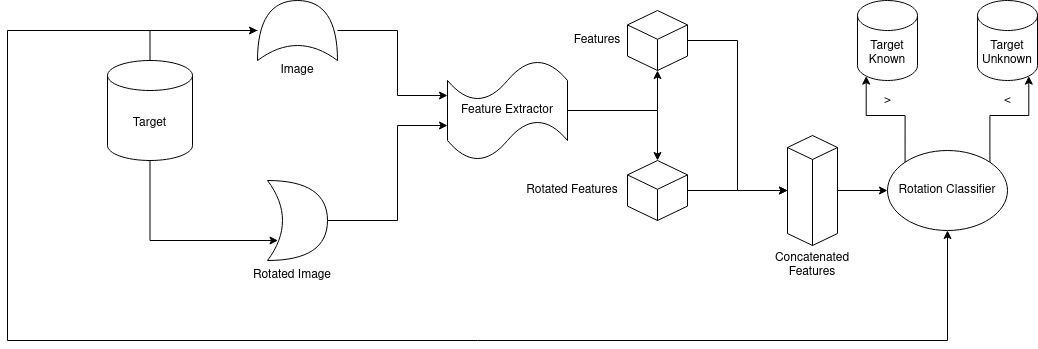
\includegraphics[width=\textwidth ]{scheme.png}
  \caption{\label{fig:separation} Schema representing the target images separation process}
\end{figure*}

In this step,
having separated the target into a known part $\mathcal{D}_t^{knw}$,
and an unknown part $\mathcal{D}_t^{unk}$,
we arrange two new datasets in order to perform the domain alignment while also learning
the unknown class.
The first one is $\mathcal{D}_s^*$, composed as $\mathcal{D}_s \cup \mathcal{D}_t^{unk}$,
which contains the original source images plus the target images identified as unknown classes.
We thus set the labels for $\mathcal{D}_t^{unk}$ as the class {\it unknown}.
The second one is $\mathcal{D}_t^{knw}$, which can be used to perform the domain alignment
without the risk of negative transfer.
While the feature extractor $E$ is inherited from the previous stage and leverages the previous training phase,
we also use two new classifiers,
$C_2$ and $R_2$.
They are similar to the previous classifiers but they have two important differences.
$C_2$ now has a $(|\mathcal{C}_s|+1)$-dimensional output to accomodate also the unknown class predictions and also
benefits from the previous learning,
while $R_2$ is always a single-head rotation classifier and starts the learning from scratch.
The training phase is the same as before with the difference that we do not have the center loss this time.
We also employ a different hyperparameter $\alpha_2$ to weigh the rotation classifier loss contribution.
The objective function is again $\mathcal{L}_2 = \mathcal{L}_{C_2} + \mathcal{L}_{R_2}$,
where the two contributions are identical to equations \ref{eq:baseloss_class} and \ref{eq:baseloss_rot}.
We report the $\mathcal{L}_{R_2}$ loss contribution to make clear the usage of $\alpha_2$ and we
recall that $\mathcal{L}_{C_2}$ is now computed using the new arranged dataset $\mathcal{D}_s^*$.

\begin{equation}
  \mathcal{L}_{R_2} = -\alpha_2\sum_{i\in\mathcal{D}_t^{knw}} {\bf z}_i^s \log \hat{{\bf z}}_i^s
  \label{eq:baseloss_rot2}
\end{equation}

\subsection{Performance metrics}
\label{sec:performance_metrics}

To have a meaningful comparison of the effectiveness
of the models to solve OSDA problems, we need to resort to a metric which
correctly measures the goodness of our predictions.
The difficulty lies on the joint presence of two, usually conflicting, goals.
We recall that an OSDA problem is characterized by the concurrent presence of
a domain difference and a class set difference.
The final goal is to correctly classify the samples belonging to known classes
while rejecting the samples of unknown classes.
The performance of both the goals are typically taken into account by two metrics, {\it OS*},
which is the fraction of the correctly classified samples belonging to known classes, and {\it UNK},
which in contrast is the accuracy over the correctly rejected samples.
Since the goals are usually conflicting, we need an overall metric which is able to correctly balance
the two contributions, providing low values if at least one of the two is low.
We therefore pick the harmonic mean of the two contributions, defined as $HOS = 2\frac{OS^*\times UNK}{OS^*+UNK}$.
We underline that $HOS$ is a more severe and fair metric to effectively measure the goodness of a model to perform well
on a given OSDA problem because, from the definition of the harmonic mean, it tends to give a bigger weight to the smaller values.

Lastly, we also exploit the AUROC metric to assess the goodness of the system in separating
the target into a known and unknown part.

\section{Experiments}
\label{sec:experiments}

\subsection{Benchmark}
\label{sec:dataset}

We evaluate the effectiveness of our proposed method exploiting the {\it Office-Home} \cite{OfficeHomeDataset} benchmark dataset,
widely used to assess the performance for OSDA settings.
The dataset is characterized by four different domains: Art (A), Clipart (C), Product (P) and Real World (R), and
each domain contains the same 65 object class categories.
We underline that the large domain gaps and the number of classes make the benchmark challenging.
For the experiments, we fix the first 45 classes (in alphabetical order) as the known classes ($\mathcal{C}_s$),
and the remaining 20 classes as the unknown ones ($\mathcal{C}_{t \setminus s}$).
For each experiment, we collect the HOS value achieved after the last training epoch of the step 2,
along with the AUROC value computed after the step 1, crucial to assess the goodness
of the system's components responsible for the separation of the target.

\subsection{Implementation Details}
\label{sec:implementation_details}

As we have already seen in section \ref{sec:method}, the network is composed of a feature extractor $E$, and two heads, $C_{1/2}$ and $R_{1/2}$.
For the feature extraction, we employ a ResNet-18\cite{ResNet18} pre-trained on ImageNet.
All the experiments are run training with a batch size equals to 32 and using a stochastic gradient descent optimization strategy
with a weight decay of 0.0005 and a momentum of 0.9.
The learning rate is set to 0.001 in the cases where we use a single-head rotation classifier as $R_1$, and 0.003 in the multi-head case.
The reason of this choice lies on the fact that, with a multi-head rotation classifier, we have to train 45 heads instead of a single one,
so the training process needs to be speeded up.
Moreover, we set a learning rate 10 times lower for the feature extractor weights.
We also decrease the learning rate using a step learning rate scheduler, which reduces it by a factor of 10 after 90\% of total epochs.
All models are trained for 50 epochs for the step one and for 25 epochs for the step two.
For models using the center loss a centroid learning rate of 0.001 is used.
The other hyperparameters are analyzed performing an ablation on section {\bf INSERT REF}.

{\it Feature extractor E}: ResNet-18 pre-trained on ImageNet. It is also shared between step 1 and step 2.

{\it Classifier $C_1$}:
It is a simple linear classifier with a 45-dimensional output.

{\it Classifier $C_2$}:
Like $C_1$ but with a 46-dimensional output to consider also the unknown class. Furthermore, it leverages the learning already performed on $C_1$.
It is worth noting that we rebalance the weight of the loss computed on samples belonging to the class unknown in the following way.
After having separated the target into $\mathcal{D}_t^{knw}$ and $\mathcal{D}_t^{unk}$,
we select the weight as $\frac{\mathcal{\bar{D}}_s}{|\mathcal{D}_t^{unk}|}$,
where ${\mathcal{\bar{D}}_s}$ is the average number of samples contained in the source known classes.
This ensures that we correctly balance the unknown class during training in a way which is independent
on the number of identified target unknown samples during the separation.

{\it Classifier $R_1$, $R_2$}: 
they are composed by a linear layer $1024\to 256$, followed by a batch normalization layer and a leaky relu activation.
The last layer is then a linear one for the actual classification $256\to 4$.
The 256-dimensional output are the features used by the center loss for inferring class centroids.
$R_2$ is always a single-head classifier, even if using a multi-head rotation classifier.

\subsection{Results}
\label{sec:results}
\begin{figure*}[h!]
  \centering
  \begin{subfigure}[b]{0.35\textwidth}
    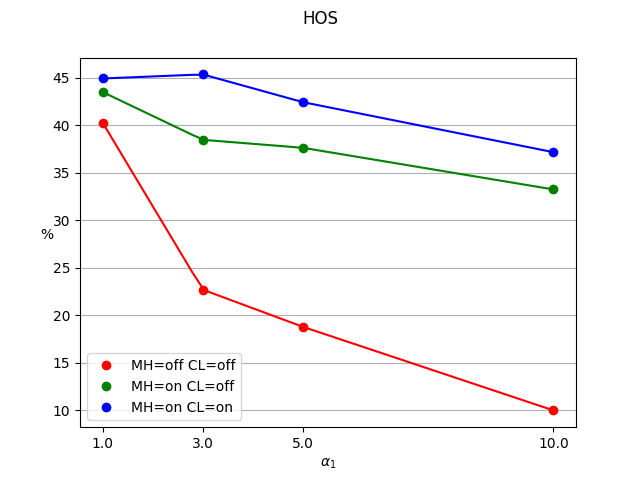
\includegraphics[trim=0 0 0 2cm, clip, width=\linewidth]{hos-a1.png}
  \end{subfigure}
  \begin{subfigure}[b]{0.35\textwidth}
    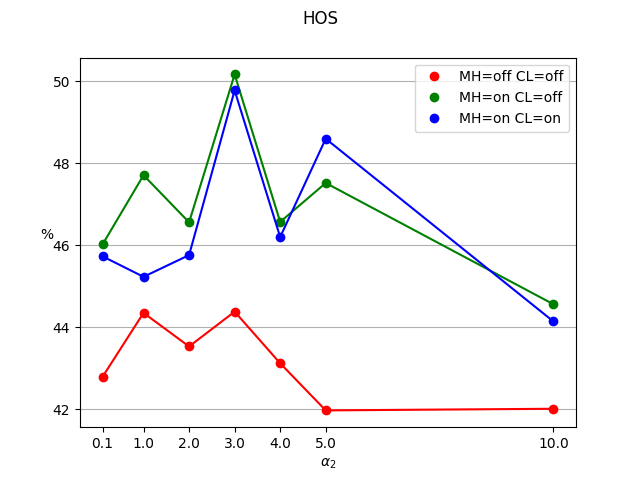
\includegraphics[trim=0 0 0 2cm, clip, width=\linewidth]{hos-a2.png}
  \end{subfigure}
  \begin{subfigure}[b]{0.35\textwidth}
    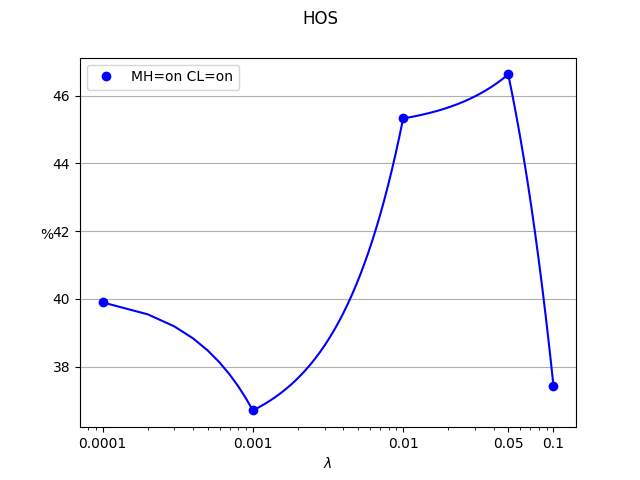
\includegraphics[trim=0 0 0 2cm, clip, width=\linewidth]{hos-l.png}
  \end{subfigure}
  \begin{subfigure}[b]{0.35\textwidth}
    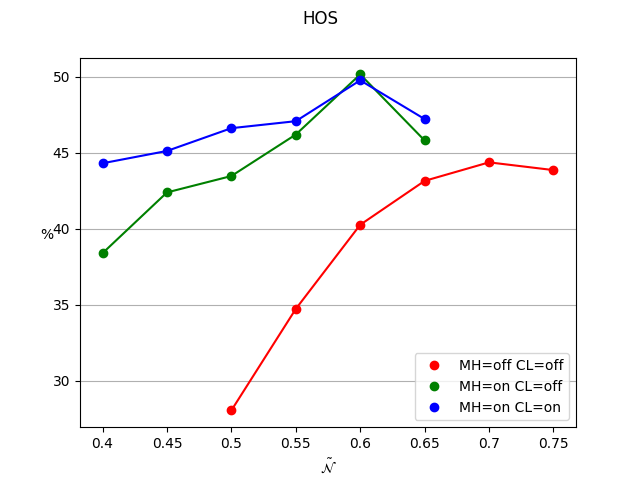
\includegraphics[trim=0 0 0 2cm, clip, width=\linewidth]{hos-th.png}
  \end{subfigure}
  \caption{\label{figurelabel} Test Caption}
\end{figure*}

Table \ref{tab:results} contains the results for all 12 available domain shifts,
as well as perfomance differences when using multi-head rotation classifiers and center loss.
Further details are to be found in section \ref{sec:implementation_details}.
We can notice that multi-headed models are more capable of correctly discriminating between known and unknown samples,
ultimately resulting in better domain alignment.
A further advantage is given when combined with center loss.
AUROC values are computed at the end of the separation stage, 
while HOS values are sampled at regular times on the entire original target dataset.

\subsection{Ablation Study}
\label{sec:ablation_study}
As shown in table \ref{tab:results} different architectures give different results, 
and as shown in table \ref{tab:params} each one requires a different set of parameters.
To choose optimal parameters a sequential approach is followed, 
by optimizing one parameter at the time.
The order of optimization followed is: 
$\alpha_1$, $\lambda_1$, $\mathcal{\tilde N}$, $\alpha_2$.
Models not using center loss just skip the $\lambda_1$ optimization.
Ablation study were run on two domain shifts, 
Art $\to$ Clipart and Clipart $\to$ Product.
In table \ref{tab:ablation_params} we report the steps followed.
All other settings follow what is reported in \ref{sec:model_parameters}.
The result here obtained are the same reported in table \ref{tab:params}.

\section{Future Work}

The results show that self-supervision technique can help in domain adaptation task and open-set classification tasks.
A few critical points still remain on our method of study and proposed solution.
The most important one is probably parameter choosing for different models, as we have seen that variations cause huge differences in results and sequential optimization of parameter is a sub-optimal heuristic.
Furthermore, having the model to learn two different tasks at once, it could be useful to use a slower learning model at the expense of longer training times.
\newpage
\appendix
\section{Test}

\begin{table}
  \centering
  \begin{tabular}[h]{||c|c|c||c||}
    \hline
    \multicolumn{4}{||c||}{OFF-OFF} \\
    \hline
    $\alpha_1$ & $\mathcal{\tilde N}$ & $\alpha_2$ & HOS$_{mean}$\\    
    \hline
    \hline
    \multicolumn{4}{||c||}{Picking $\alpha_1$} \\
    \hline
    {\bf 1.0}  & \multirow{4}{*}{0.6} & \multirow{4}{*}{3.0} & {\bf 40.27\%} \\
    3.0  & & & 22.69\% \\
    5.0  & & & 18.78\% \\
    10.0 & & & 9.99\% \\
    \hline
    \hline
    \multicolumn{4}{||c||}{Picking $\mathcal{\tilde N}$} \\
    \hline
    \multirow{4}{*}{1.0} & 0.50 & \multirow{4}{*}{3.0}  & 28.05\%\\
    & 0.55 & & 34.73\% \\
    & 0.60 & & 40.27\% \\
    & 0.65 & & 43.16\% \\
    \hline
    \hline
    \multicolumn{4}{||c||}{Picking $\alpha_2$} \\
    \hline
    \multirow{7}{*}{1.0} & \multirow{7}{*}{0.7} & 0.1 & 42.79\%\\
    && 1.0 & 44.35\% \\
    && 2.0 & 43.53\% \\
    && {\bf 3.0} & {\bf 44.38}\% \\
    && 4.0 & 43.12\% \\
    && 5.0 & 41.97\% \\
    && 10.0 & 42.01\% \\
    \hline
  \end{tabular}
  \caption{\centering\label{tab:ablationoffoff} Hyperparameters picking process for configuration Multi-Head Off and Center-Loss Off}
\end{table}



\begin{table}
  \centering
  \begin{tabular}[h]{||c|c|c||c||}
    \hline
    \multicolumn{4}{||c||}{ON-OFF} \\
    \hline
    $\alpha_1$ & $\mathcal{\tilde N}$ & $\alpha_2$ & HOS$_{mean}$\\    
    \hline
    \hline
    \multicolumn{4}{||c||}{Picking $\alpha_1$} \\
    \hline
    {\bf 1.0}  & \multirow{4}{*}{0.6} & \multirow{4}{*}{3.0} & {\bf 43.48\%} \\
    3.0  & & & 38.45\% \\
    5.0  & & & 37.61\% \\
    10.0 & & & 33.23\% \\
    \hline
    \hline
    \multicolumn{4}{||c||}{Picking $\mathcal{\tilde N}$} \\
    \hline
    \multirow{6}{*}{1.0} & 0.4 & \multirow{6}{*}{3.0}  & 38.40\%\\
    & 0.45 & & 42.40\% \\
    & 0.5 & & 43.48\% \\
    & 0.55 & & 46.21\% \\
    & {\bf0.6} & & {\bf 50.17\%} \\
    & 0.65 & & 45.82\% \\
    \hline
    \hline
    \multicolumn{4}{||c||}{Picking $\alpha_2$} \\
    \hline
    \multirow{7}{*}{1.0} & \multirow{7}{*}{0.7} & 0.1 & 46.02\%\\
    && 1.0 & 47.71\% \\
    && 2.0 & 46.56\% \\
    && {\bf 3.0} & {\bf 50.17\%} \\
    && 4.0 & 46.57\% \\
    && 5.0 & 47.52\% \\
    && 10.0 & 44.56\% \\
    \hline
  \end{tabular}
  \caption{\centering\label{tab:ablationonoff} Hyperparameters picking process for configuration Multi-Head On and Center-Loss Off}
\end{table}


\begin{table}
  \centering
  \begin{tabular}[h]{||c|c|c|c||c||}
    \hline
    \multicolumn{5}{||c||}{ON-ON} \\
    \hline
    $\alpha_1$ & $\lambda_1$ & $\mathcal{\tilde N}$ & $\alpha_2$ & HOS$_{mean}$ \\
    \hline
    \hline
    \multicolumn{5}{||c||}{Picking $\alpha_1$} \\
    \hline
    1.0 & \multirow{4}{*}{0.01} & \multirow{4}{*}{0.05} & \multirow{4}{*}{3.0} & 44.90\% \\
    {\bf 3.0} & && & {\bf 45.33\%} \\
    5.0 & && & 42.41\% \\
    10.0 & && & 37.15\% \\
    \hline
    \hline
    \multicolumn{5}{||c||}{Picking $\lambda_1$} \\
    \hline
    \multirow{5}{*}{3} & 0.0001 & \multirow{5}{*}{0.5} & \multirow{5}{*}{3.0} & 39.90\% \\
    & 0.001 & & & 36.71\% \\
    & 0.01 & & & 45.33\% \\
    & {\bf 0.05 }& & & {\bf 46.63\%} \\
    & 0.1 & & & 37.44\% \\
    \hline
    \hline
    \multicolumn{5}{||c||}{Picking $\mathcal{\tilde N}$} \\
    \hline
    \multirow{5}{*}{3} & \multirow{5}{*}{0.05} & 0.4 & \multirow{5}{*}{3.0} & 44.32\% \\
    & & 0.45 & & 45.13\% \\
    & & 0.5 & & 46.63\% \\
    & & 0.55 & & 47.09\% \\
    & & {\bf 0.6} & & {\bf 49.78\%} \\
    \hline
    \hline
    \multicolumn{5}{||c||}{Picking $\alpha_2$} \\
    \hline
    \multirow{7}{*}{3} & \multirow{7}{*}{0.05} & \multirow{7}{*}{0.6} & 0.1 & 45.73\% \\
    & & & 1.0 & 45.23\% \\
    & & & 2.0 & 45.76\% \\
    & & & {\bf 3.0} & {\bf 49.78\%} \\
    & & & 4.0 & 46.20\% \\
    & & & 5.0 & 48.60\% \\
    & & & 10.0 & 44.14\% \\
    \hline
  \end{tabular}
  \caption{\centering\label{tab:ablationonon} Hyperparameters picking process for configuration Multi-Head On and Center-Loss On}
\end{table}


\begin{table}
  \centering
  \begin{tabular}[t]{||c|c|c||c|c||}
    \hline
    \multicolumn{5}{||c||}{Single-Head, CE Loss} \\
    \hline
    Source & Target & AUROC & HOS & HOS* \\
    S & T & 50\% & 30\% & 30\% \\
    S & T & 50\% & 30\% & 30\% \\
    S & T & 50\% & 30\% & 30\% \\
    \hline
    \hline
    \multicolumn{5}{||c||}{Multi-Head, CE Loss} \\
    \hline
    Source & Target & AUROC & HOS & HOS* \\
    S & T & 50\% & 30\% & 30\% \\
    S & T & 50\% & 30\% & 30\% \\
    S & T & 50\% & 30\% & 30\% \\
    \hline
    \hline
    \multicolumn{5}{||c||}{Single-Head, CE+C Loss} \\
    \hline
    Source & Target & AUROC & HOS & HOS* \\
    S & T & 50\% & 30\% & 30\% \\
    S & T & 50\% & 30\% & 30\% \\
    S & T & 50\% & 30\% & 30\% \\
    \hline
    \hline
    \multicolumn{5}{||c||}{Multi-Head, CE+C Loss} \\
    \hline
    Source & Target & AUROC & HOS & HOS* \\
    S & T & 50\% & 30\% & 30\% \\
    S & T & 50\% & 30\% & 30\% \\
    S & T & 50\% & 30\% & 30\% \\
    \hline 
    \hline
    \multicolumn{5}{||c||}{No Rotation} \\
    \hline
    Source & Target & AUROC & HOS & HOS$_{Best}$ \\
    S & T & 50\% & 30\% & 30\% \\
    S & T & 50\% & 30\% & 30\% \\
    S & T & 50\% & 30\% & 30\% \\
    \hline
  \end{tabular}
  \caption{\centering\label{tab:results}Results for domain alignment. AUROC is the area under the ROC. HOS is latest achieved HOS, HOS* the best achieved through all epochs.}
\end{table}


%%%%%%%%% REFERENCES
{\small
\bibliographystyle{ieee_fullname}
\bibliography{egbib}
}

\end{document}
